\chapter{IceCube Neutrino Observatory} \label{sec:icecube}

Because of the small cross section of neutrinos, a huge detection volume is needed to detect these particles in a statistically sufficient quantity \cite{cross_n}.
Since the detection of neutrinos is based on the Cherenkov radiation of secondary particles, a detection medium is needed that is transparent to radiation in this range.
With regard to these two problems, the kilometer-thick ice at the south pole is a good choice.
The resulting IceCube neutrino observatory is the world's largest particle detector.
It is almost exactly located at the southernmost point of the earth and shown schematically in figure \ref{fig:icecube}.

\begin{figure}
    \centering
    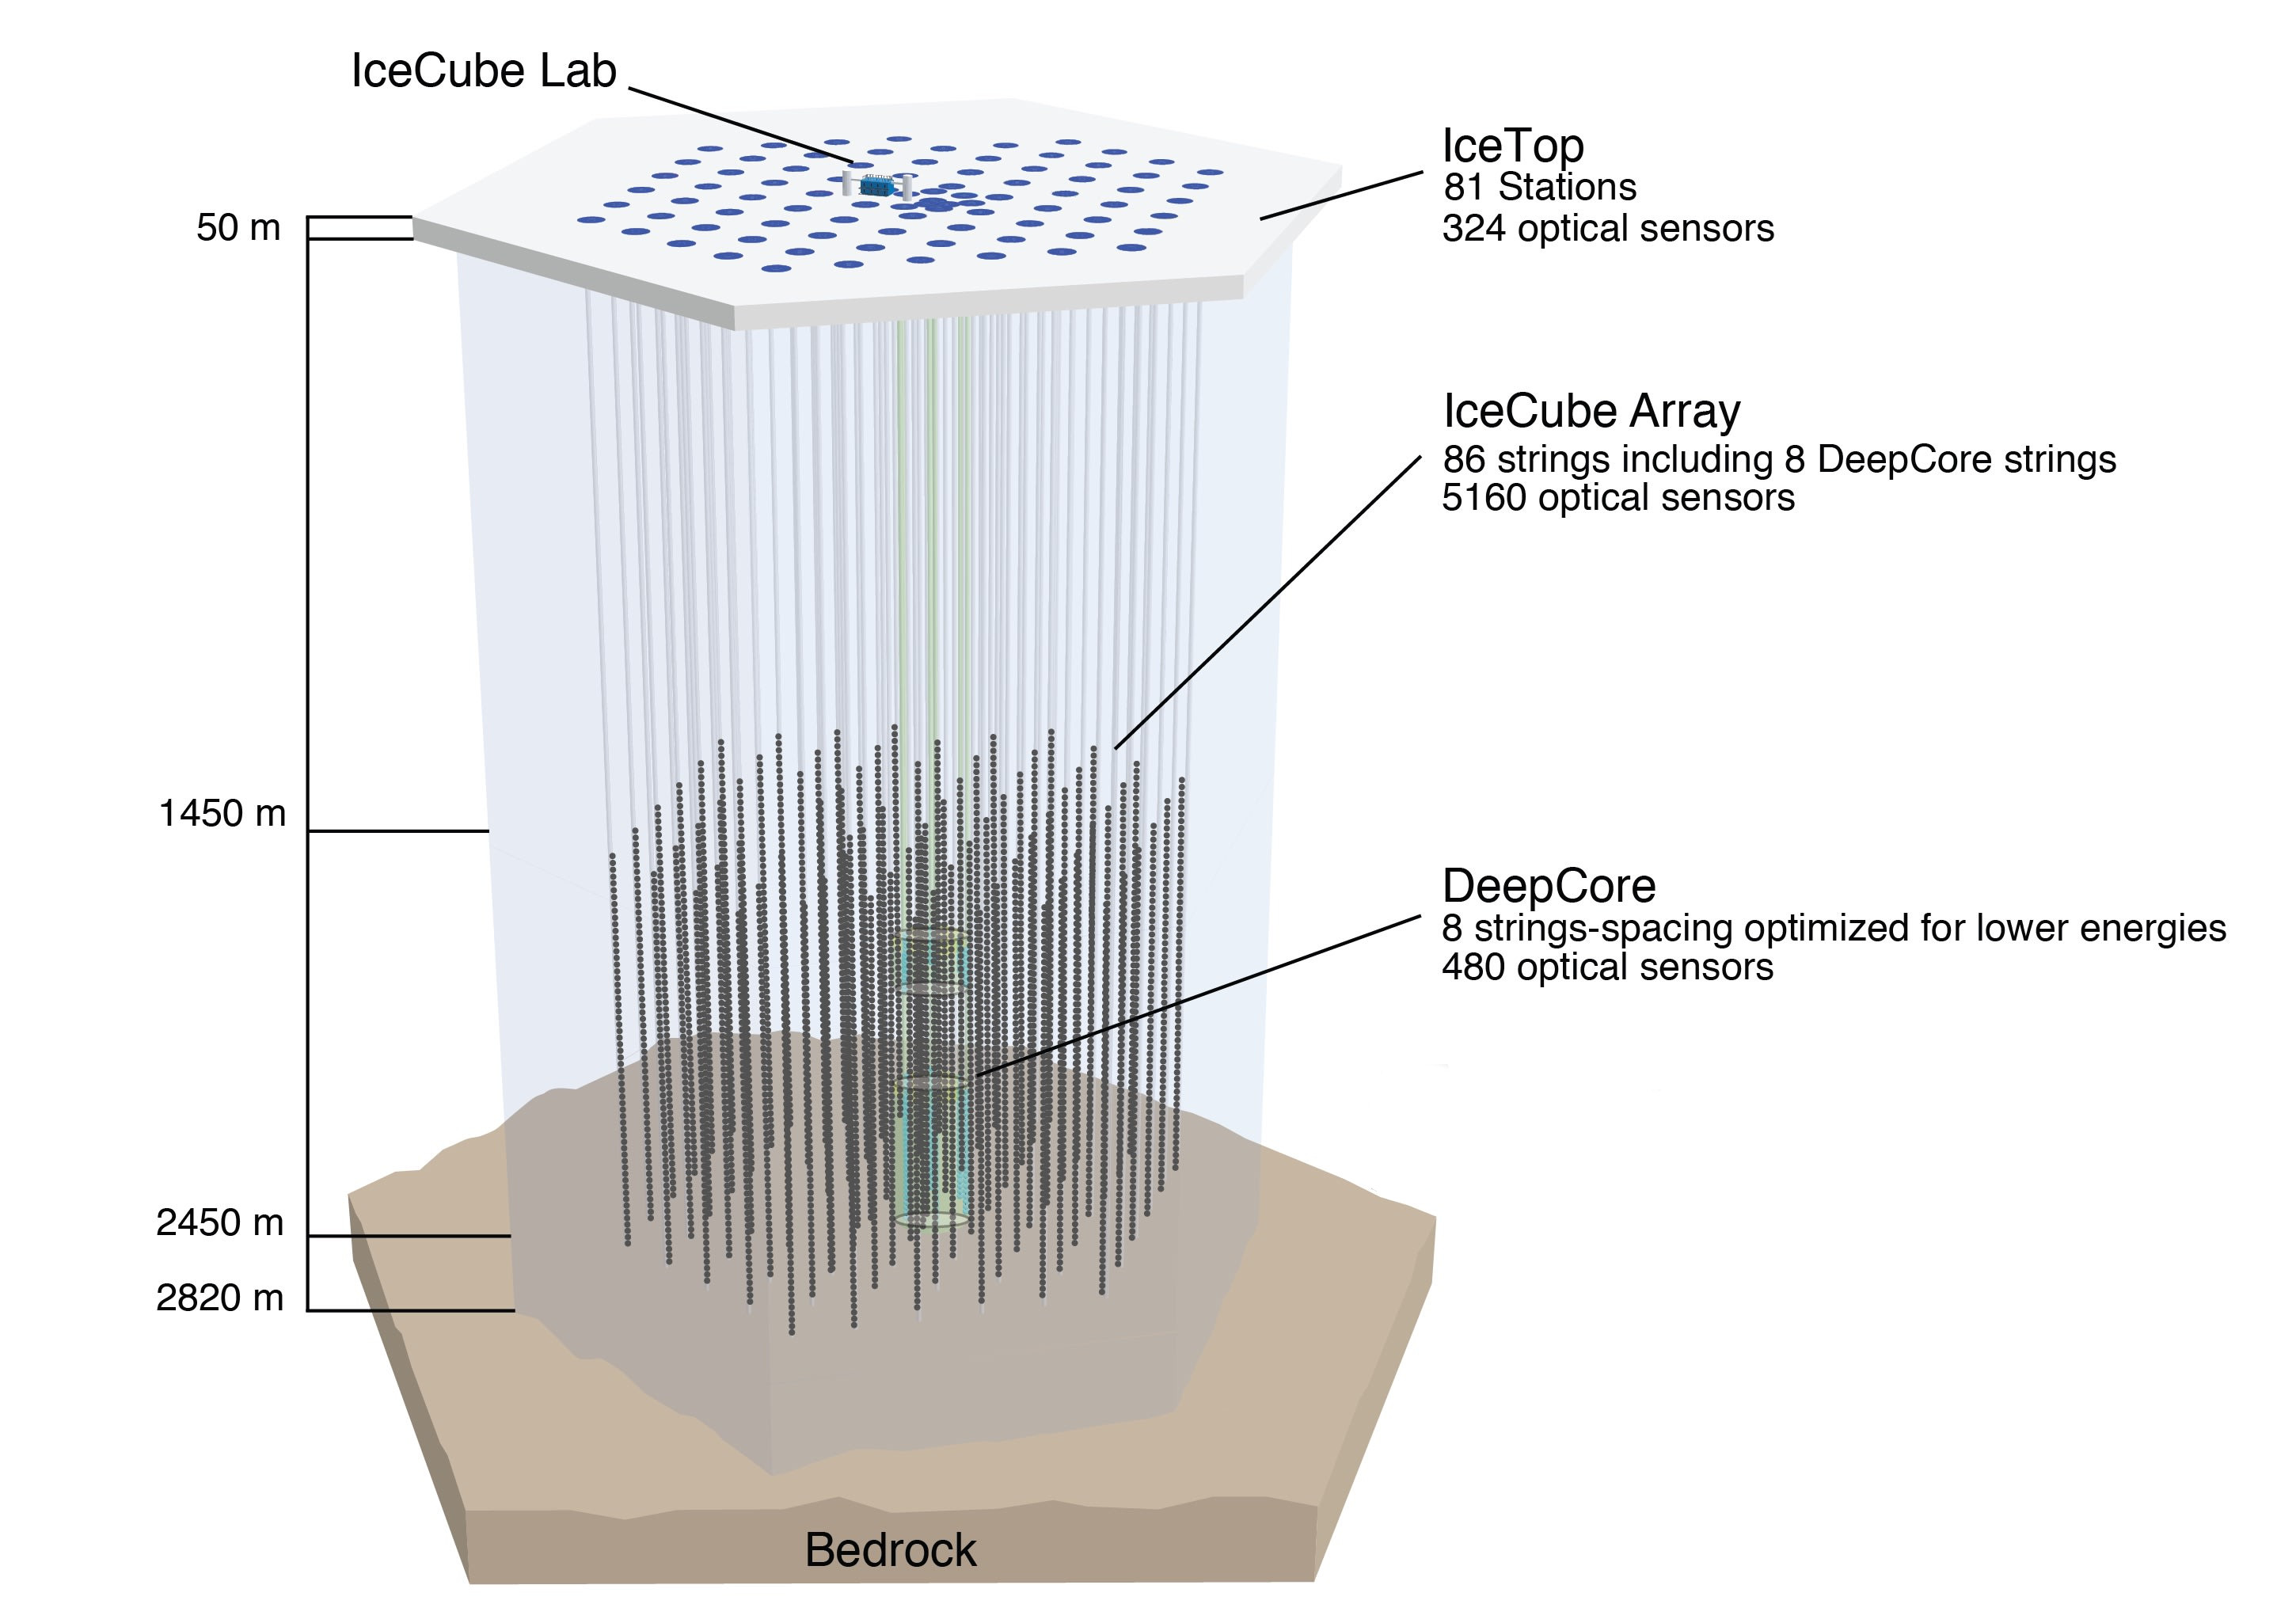
\includegraphics[width=\linewidth]{Plots/01_7_icecube/IceCube-Array.jpg}
    \caption{Schematic representation of the IceCube detector \cite{icecube_website}.}
    \label{fig:icecube}
\end{figure}

Its construction started in $\num{2004}$ and took $\num{7}$ years to its completion in $\num{2010}$.
The detector volume of IceCube covers about $\SI{1}{\kilo\meter\tothe{3}}$ of clear antarctic ice.
$\num{86}$ holes were drilled into the ice to let down cables with $\num{60}$ digital optical modules (DOMs) each.
The detection volume, or the position of the first DOM respectively, starts at a depth of about $\SI{1450}{\meter}$ and ends in a depth of about $\SI{2450}{\meter}$.
The area known as the DeepCore in the middle of the detector features a denser collection of DOMs.
IceCube detects about $\num{275}$ million cosmic rays and $\num{275}$ atmospheric neutrinos every day \cite{icecube_website}.

\section{Detection Principle}

When neutrinos interact with a medium, charged secondary particles are produced.
this occurs through a neutral current (NC) via a $Z^0$ boson or through a charged current (CC) via a $W$ boson
\begin{equation}
  \nu_l + N \rightarrow Z^0 \rightarrow \nu^{\prime}_l + X \text{ and }  \nu_l + N \rightarrow W \rightarrow l + X, \label{eq:nc_cc_int}
\end{equation}
with $N$ and $X$ being nuclei before and after the interaction \cite{Ahlers_2018}.
If the charged secondary particles (the charged leptons $l$ in \eqref{eq:nc_cc_int}) now move through a medium at a speed faster than the speed of light in the medium, the charged secondary particles polarise the atoms along the direction of flight for a short time.
The resulting light is called Cherenkov light and is emitted at an angle of
\begin{equation}
  \Theta = \arccos{\left(\frac{1}{\beta n}\right)}, \label{eq:cherenkov}
\end{equation}
with the relativistic velocity $\beta=v/c$ of the particle and the refractive index of the medium $n$ \cite{PhysRev52378,spiering}.
A schematic representation of the Cherenkov effect is given in Figure \ref{fig:cherenkov}.
This leads to the emergence of two event signatures in the detector volume, tracks and cascades.
Tracks are produced by charged current interactions and gain their signature by the energy loss of the primary charged lepton and the secondary particles via ionization, bremsstrahlung, pair production and photo-nuclear interactions in the ice.
Cascades are created by both charged current and neutral current interactions and get their traditional signature from the rapid decay and extreme scattering of secondary particles.
\begin{figure}
  \centering
  \scalebox{0.5}{
  \begin{tikzpicture}[scale=1,
    >=stealth',
    pos=.8,
    photon/.style={decorate,decoration={snake,post length=1mm}},
    declare function={
    x1 = (sqrt(25-5*sin(45)));
    x2 = 10;
    y1 = 5*sin(45);
    y2 = 0;
    m = (5*sqrt(2)/(-20+sqrt(100-10*sqrt(2))));
    b =  (-50*sqrt(2)/(-20+sqrt(100-10*sqrt(2))));
    o = 0.5 * sqrt(25-5*sin(45));
    p = 0.5*5*sin(45);
    }
    ]
    %\draw[thick] (-3,0) -- (0,0);
    %triangle
    \draw[thick] (0,0) -- (10,0) -- (sqrt{25-5*sin{45}},5*sin{45}) -- cycle;
    \draw[thick] (0,0) -- (10,0) -- (sqrt{25-5*sin{45}},-5*sin{45});
    \draw[thick] ([shift=(0:1cm)]0,0) arc (0:67:1cm);
    \draw[thick] ([shift=(-113:1cm)]sqrt{25-5*sin{45}},5*sin{45}) arc (-113:-23:1cm);
    \node at (0.5,0.4) {$\Theta$};
    \node[mark size=1pt] at (sqrt{25-5*sin{45}} + 0.25,5*sin{45} - 0.53) {\pgfuseplotmark{*}};
    \node[scale=2] at (0.2,0.5*5*sin{45}) {$\frac{c}{n}$};
    \node[below,scale=2] at (4.5,-0.2) {$v$};
    %circles
    \draw[teal, thick] (0,0) circle (3.82);
    \draw[teal, thick] (4,0) circle (2.28);
    \draw[teal, thick] (6.5,0) circle (1.32);
    \draw[teal, thick] (8,0) circle (0.75);
    %particles
    \draw[teal,thick, ->] (10,0) -- (11,0);
    \node[mark size=2pt,teal] at (10,0) {\pgfuseplotmark{*}};
    \node[teal,scale=2] at (10,1) {$l$};
    \draw[thick,blue,photon, ->] (sqrt{25-5*sin{45}},5*sin{45}) -- node[below right,scale=2] {$\gamma$} (sqrt{25-5*sin{45}}+0.6,5*sin{45}+1.3);
    \draw[thick,blue,photon, ->] (4.9,2.1) -- (4.9+0.6,2.1+1.3);
    \draw[thick,blue,photon, ->] (7,1.25) -- (7+0.6,1.25+1.3);
    \draw[thick,blue,photon, ->] (8.3,0.7) -- (8.3+0.6,0.7+1.3);
    \draw[thick,blue,photon, ->] (sqrt{25-5*sin{45}},-5*sin{45}) -- (sqrt{25-5*sin{45}}+0.6,-5*sin{45}-1.3);
    \draw[thick,blue,photon, ->] (4.9,-2.1) -- (4.9+0.6,-2.1-1.3);
    \draw[thick,blue,photon, ->] (7,-1.25) -- (7+0.6,-1.25-1.3);
    \draw[thick,blue,photon, ->] (8.3,-0.7) -- (8.3+0.6,-0.7-1.3);
    %\draw[thick,blue,->] (sqrt{25-5*sin{45}},5*sin{45}) -- (sqrt{25-5*sin{45}}+0.5*sqrt{25-5*sin{45}},5*sin{45}+0.5*5*sin{45});
    %\draw[thick,blue,->] (sqrt{25-5*sin{45}},m*x1+b) -- (sqrt{25-5*sin{45}}+0.5*sqrt{25-5*sin{45}},m*x1+b+0.5*5*sin{45});%(5,y*(5-sqrt{25-5*sin{45}})) -- (0,0);%(5+0.2*sqrt{25-5*sin{45}},y*(5-sqrt{25-5*sin{45}}+0.2*5*sin{45}));
  \end{tikzpicture}}
  \caption{Schematic visualisation of the Cherenkov radiation $\gamma$ emitted by a charged lepton $l$ traveling with velocity $v>c/n$ through a medium with a refractive index $n$ polarizing the medium on its way. The resulting cone of Cherenkov radiation is visually comparable to the supersonic cone of an aeroplane.}
  \label{fig:cherenkov}
\end{figure}

\section{Tracks and Cascades}

To perform a point source search, two properties of the detector signatures of the muons are of particular importance: the direction and the energy.
It is therefore important to distinguish between two types of events, tracks and cascades.
Tracks pass through the detector but do not deposit all their energy in the detector volume.
This means that the direction of the event can be reconstructed very well.
The signature left by such an event can be seen in figure \ref{fig:track}.
However, since the total energy is not deposited in the detector volume, the reconstruction of the energy is generally not optimal.
\begin{figure}
    \centering
    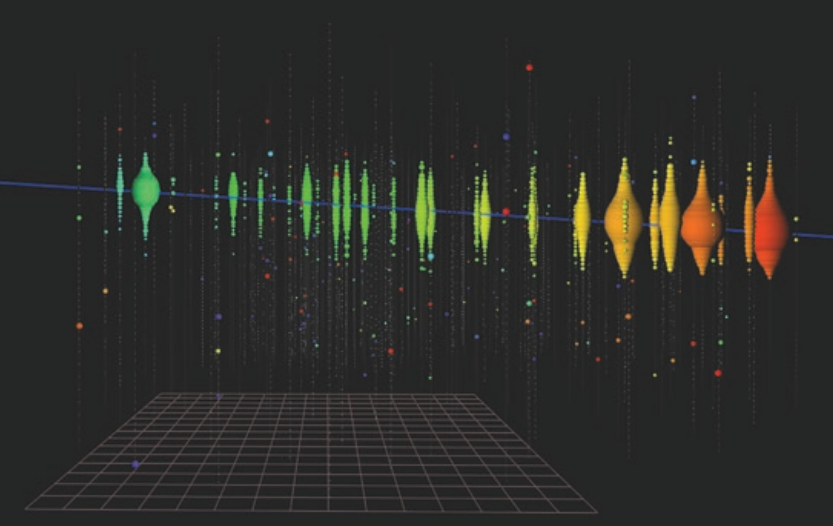
\includegraphics[width=10cm]{Plots/01_7_icecube/track.png}
    \caption{Tracklike event signature in the detectorvolume. The deposited energy is represented by the size of the spheres, the time of arrival by the colour (red earlier, blue later). The small glow of individual modules is unfiltered noise \cite{spiering}.}
    \label{fig:track}
\end{figure}

Cascades, on the other hand, deposit their entire energy in the detector volume, which means that the energy can be determined quite accurately.
Due to the shape of the cascade event, however, the original direction is very difficult to reconstruct.
Such an event can be seen in figure \ref{fig:cascade}.
Generally, the magnitude of the event's energy is the main statistical indicator of whether an event is astrophysical in origin, but the exact reconstruction of the event's direction is very important for a point source search.
Therefore, a dataset from tracks is usually used.
However, due to their high energy, cascade events can be used as a source catalogue \cite{steve_und_mirco}, but this is not the case in this thesis.
\begin{figure}
    \centering
    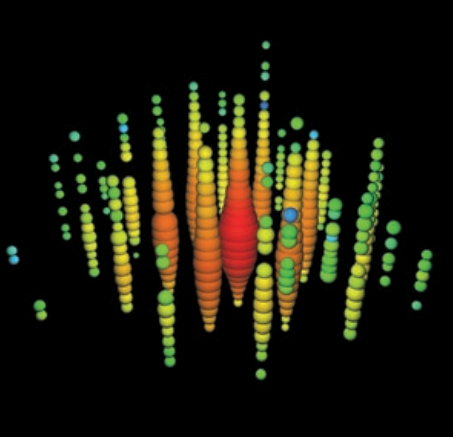
\includegraphics[width=10cm]{Plots/01_7_icecube/cascade.png}
    \caption{The filtered cascade event nicknamed \textit{Ernie} with a reconstructed energy of $\SI{1.04}{\peta\electronvolt}$. The deposited energy is represented by the size of the spheres, the time of arrival by the colour (red earlier, blue later) \cite{spiering}.}
    \label{fig:cascade}
\end{figure}
